\documentclass[9pt,twocolumn,twoside,lineno]{pnas-new}
% Use the lineno option to display guide line numbers if required.

\templatetype{pnasresearcharticle} % Choose template 
% {pnasresearcharticle} = Template for a two-column research article
% {pnasmathematics} %= Template for a one-column mathematics article
% {pnasinvited} %= Template for a PNAS invited submission

\title{Biomechanical trade-offs in the pelvic floor constrain the evolution of the human birth canal}

% Use letters for affiliations, numbers to show equal authorship (if applicable) and to indicate the corresponding author
\author[a,1]{Ekaterina Stansfield}
\author[b]{Krishna Kumar} 
\author[a,c]{Philipp Mitteroecker}
\author[c,a,d,1]{Nicole D.S. Grunstra}

\affil[a]{Department of Evolutionary Biology, University of Vienna, Vienna, Austria 1090}
\affil[b]{Department of Civil, Architectural and Environmental Engineering, Cockrell School of Engineering, University of Texas at Austin, Austin, Texas 78712-0273, USA.}
\affil[c]{Konrad Lorenz Institute for Evolution and Cognition Research, Klosterneuburg, Austria 3400.}
\affil[d]{Mammal Collection, Natural History Museum Vienna, Vienna, Austria 1010.}

% Please give the surname of the lead author for the running footer
\leadauthor{Stansfield} 

% Please add a significance statement to explain the relevance of your work

% Please add a significance statement to explain the relevance of your work
\significancestatement{The relatively small human birth canal has arisen from an
	evolutionary trade-off between multiple antagonistic selective forces. We present evidence that a large pelvic floor is disadvantageous for maintaining continence and supporting the weight of the inner organs and the fetus through multiple finite element analyses of pelvic floor models varying in size and thickness. An increase in pelvic floor size led to a disproportionately large deflection as well as higher tissue stretches and stresses. Increased pelvic floor thickness considerably reduced
	deflection by increasing stiffness. However, as a side effect, it increases the intra-abdominal pressure necessary for childbirth, thus reflecting another evolutionary trade-off affecting not only the size but also the thickness of the pelvic floor.}

% Please include corresponding author, author contribution and author declaration information
\authorcontributions{All authors contributed to the conception and design of the research. ES created the FE models and ran the experiments. ES and KK analyzed the data. All authors critically interpreted the results and all authors drafted and critically revised the manuscript.}
\authordeclaration{Authors have no competing interests.}
\equalauthors{\textsuperscript{1} Co-corresponding Authors.  katya.stansfield\@univie.ac.at and nicolegrunstra\@gmail.com}
%\correspondingauthor{\textsuperscript{2}To whom correspondence should be addressed. }

% At least three keywords are required at submission. Please provide three to five keywords, separated by the pipe symbol

\keywords{pelvic floor $|$ human birth canal $|$ biomechanics $|$ evolutionary trade-off $|$ finite element modeling} 

\begin{abstract}
Compared to most other primates, humans are characterized by a tight fit between the maternal birth canal and the fetal head, leading to a relatively high risk of neonatal and maternal mortality and morbidities. Obstetric selection is thought to favor a spacious birth canal, whereas the source for opposing selection is frequently assumed to relate to bipedal locomotion. An alternative, yet under-investigated, hypothesis is that a more expansive birth canal suspends the soft tissue of the pelvic floor across a larger area, which is disadvantageous for continence and support of the weight of the inner organs and fetus. To test this ‘pelvic floor hypothesis’ we generated a finite element model of the human female pelvic floor and varied its radial size and thickness while keeping all else constant. This allowed us to study the effect of pelvic geometry on pelvic floor deflection (i.e., the amount of bending from the original position) and tissue stresses and stretches. Deflection grew disproportionately fast with increasing radial size, and stresses and stretches also increased. By contrast, an increase in thickness increased pelvic floor stiffness - i.e. the resistance to deformation - which reduced deflection but was unable to fully compensate for the effect of increasing radial size. Moreover, larger thicknesses increase the intra-abdominal pressure necessary for childbirth. Our results support the pelvic floor hypothesis and evince functional trade-offs affecting not only the size of the birth canal but also the thickness and stiffness of the pelvic floor.
\end{abstract}

\dates{This manuscript was compiled on \today}
\doi{\url{https://doi.org/10.1073/pnas.2022159118}}

\begin{document}

\maketitle
\thispagestyle{firststyle}
\ifthenelse{\boolean{shortarticle}}{\ifthenelse{\boolean{singlecolumn}}{\abscontentformatted}{\abscontent}}{}

% If your first paragraph (i.e. with the \dropcap) contains a list environment (quote, quotation, theorem, definition, enumerate, itemize...), the line after the list may have some extra indentation. If this is the case, add \parshape=0 to the end of the list environment.
\section*{Introduction}
\dropcap{H}umans are characterized by a close match (and occasional mismatch) between the dimensions of the maternal bony pelvis and fetal size. This tight fetopelvic fit leads to a comparatively difficult birth process in humans. Without medical intervention, fetopelvic disproportion often leads to maternal and neonatal death. Birth-related morbidities such as pelvic organ prolapse (i.e., the pathological descent of organs into or through the vagina or rectum) and incontinence affect millions of women worldwide, which can have serious social and health consequences~\cite{Arrowsmith1996-jn}. In western countries, a quarter to more than half of women report suffering from one or more pelvic floor disorders, with the reported prevalence of urinary incontinence ranging from 15\% to 69\% and of prolapse ranging from 6\% to 41\% 2–5. Although their prevalence increases with age and parity, pelvic floor disorders are also common among young and nulliparous women 4–6. Understanding the evolutionary origins of obstructed labor thus is a pressing and highly debated challenge 7–12.
	

\section*{Guide to using this template on Overleaf}

Please note that whilst this template provides a preview of the typeset manuscript for submission, to help in this preparation, it will not necessarily be the final publication layout. For more detailed information please see the \href{ https://www.pnas.org/page/authors/format}{PNAS Information for Authors}.

If you have a question while using this template on Overleaf, please use the help menu (``?'') on the top bar to search for \href{https://www.overleaf.com/help}{help and tutorials}. You can also \href{https://www.overleaf.com/contact}{contact the Overleaf support team} at any time with specific questions about your manuscript or feedback on the template.

\subsection*{Author Affiliations}

Include department, institution, and complete address, with the ZIP/postal code, for each author. Use lower case letters to match authors with institutions, as shown in the example. PNAS strongly encourages authors to supply an \href{https://orcid.org/}{ORCID identifier} for each author. Individual authors must link their ORCID account to their PNAS account at \href{http://www.pnascentral.org/}{www.pnascentral.org}. For proper authentication, authors must provide their ORCID at submission and are not permitted to add ORCIDs on proofs.

\subsection*{Submitting Manuscripts}

All authors must submit their articles at \href{http://www.pnascentral.org/cgi-bin/main.plex}{PNAScentral}. If you are using Overleaf to write your article, you can use the ``Submit to PNAS'' option in the top bar of the editor window. 

\subsection*{Format}

Many authors find it useful to organize their manuscripts with the following order of sections; title, author line and affiliations, keywords, abstract, introduction, results, discussion, materials and methods, acknowledgments, and references. Other orders and headings are permitted.

\subsection*{Manuscript Length}

Brief Reports are limited to 3 pages, which is approximately 1,600 words (including the manuscript text, title page, abstract, and figure legends), and 15 references. Supporting information (SI) is limited to extended methods, essential supporting datasets, and videos (no additional tables or figures).


\subsection*{References}

References should be cited in numerical order as they appear in text; this will be done automatically via bibtex, e.g. \cite{belkin2002using} and \cite{berard1994embedding,coifman2005geometric}. All references cited in the main text should be included in the main manuscript file.  

\subsection*{Data Archival}

PNAS must be able to archive the data essential to a published article. Where such archiving is not possible, deposition of data in public databases, such as GenBank, ArrayExpress, Protein Data Bank, Unidata, and others outlined in the \href{https://www.pnas.org/page/authors/journal-policies#xi}{Information for Authors}, is acceptable.

\subsection*{Language-Editing Services}
Prior to submission, authors who believe their manuscripts would benefit from professional editing are encouraged to use a language-editing service (see list at www.pnas.org/page/authors/language-editing). PNAS does not take responsibility for or endorse these services, and their use has no bearing on acceptance of a manuscript for publication. 

\begin{figure}%[tbhp]
\centering
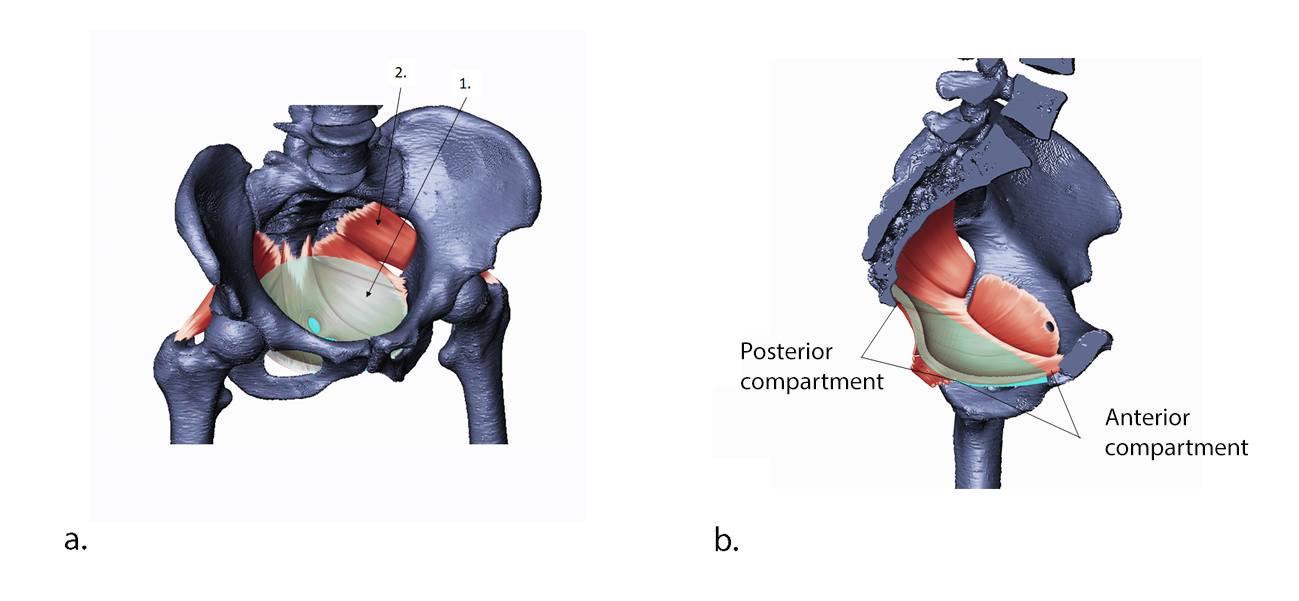
\includegraphics[width=\linewidth]{figs/fig1}
\caption{Placeholder image of a frog with a long example legend to show justification setting.}
\label{fig:frog}
\end{figure}


\begin{SCfigure*}[\sidecaptionrelwidth][t]
\centering
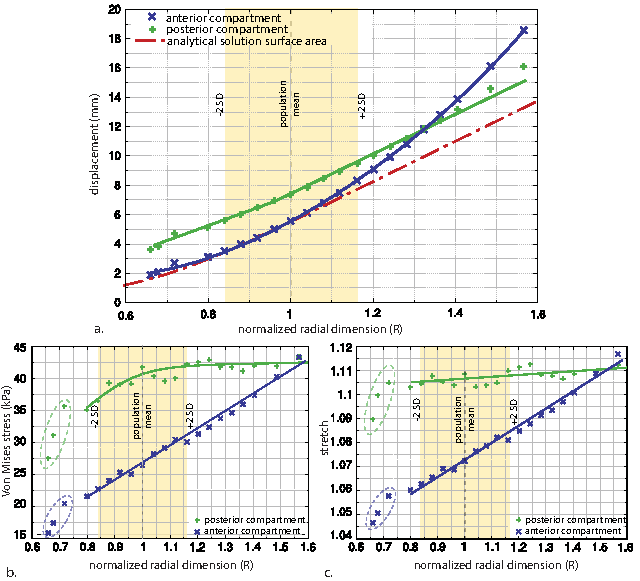
\includegraphics[width=.8\linewidth]{figs/fig2}
\caption{This legend would be placed at the side of the figure, rather than below it.}\label{fig:side}
\end{SCfigure*}

\subsection*{Digital Figures}

EPS, high-resolution PDF, and PowerPoint are preferred formats for figures that will be used in the main manuscript. Authors may submit PRC or U3D files for 3D images; these must be accompanied by 2D representations in TIFF, EPS, or high-resolution PDF format. Color images must be in RGB (red, green, blue) mode. Include the font files for any text.

Images must be provided at final size, preferably 1 column width (8.7cm). Figures wider than 1 column should be sized to 11.4cm or 17.8cm wide. Numbers, letters, and symbols should be no smaller than 6 points (2mm) and no larger than 12 points (6mm) after reduction and must be consistent.

Figures and tables should be labelled and referenced in the standard way using the \verb|\label{}| and \verb|\ref{}| commands.

Figure \ref{fig:frog} shows an example of how to insert a column-wide figure. To insert a figure wider than one column, please use the \verb|\begin{figure*}...\end{figure*}| environment. Figures wider than one column should be sized to 11.4 cm or 17.8 cm wide. Use \verb|\begin{SCfigure*}...\end{SCfigure*}| for a wide figure with side legends.

\subsection*{Tables}
Tables should be included in the main manuscript file and should not be uploaded separately.

\subsection*{Single column equations}

Authors may use 1- or 2-column equations in their article, according to their preference.

To allow an equation to span both columns, use the \verb|\begin{figure*}...\end{figure*}| environment mentioned above for figures.

Note that the use of the \verb|widetext| environment for equations is not recommended, and should not be used. 

\begin{figure*}[bt!]
\begin{align*}
(x+y)^3&=(x+y)(x+y)^2\\
       &=(x+y)(x^2+2xy+y^2) \numberthis \label{eqn:example} \\
       &=x^3+3x^2y+3xy^3+x^3. 
\end{align*}
\end{figure*}


\begin{table}%[tbhp]
\centering
\caption{Comparison of the fitted potential energy surfaces and ab initio benchmark electronic energy calculations}
\begin{tabular}{lrrr}
Species & CBS & CV & G3 \\
\midrule
1. Acetaldehyde & 0.0 & 0.0 & 0.0 \\
2. Vinyl alcohol & 9.1 & 9.6 & 13.5 \\
3. Hydroxyethylidene & 50.8 & 51.2 & 54.0\\
\bottomrule
\end{tabular}

\addtabletext{nomenclature for the TSs refers to the numbered species in the table.}
\end{table}

\subsection*{Supporting Information (SI)}

Authors are limited to the following types of SI: extended methods, datasets, videos, and 3D figures. Extended discussion is not permitted.

\subsection*{SI Appendix}

Supply extended materials and methods information in a separate SI Appendix PDF file. Include SI movie legends. SI will be published as provided by the authors; it will not be edited or composed. Supplementary figures and tables are not allowed.


\subsubsection*{SI Datasets} 

Supply .xlsx, .csv, .txt, .rtf, or .pdf files. This file type will be published in raw format and will not be edited or composed.


\subsubsection*{SI Movies}

Supply Audio Video Interleave (avi), Quicktime (mov), Windows Media (wmv), animated GIF (gif), or MPEG files and and include a brief legend for each movie in the main manuscript file. All movies should be submitted at the desired reproduction size and length. Movies should be no more than 10 MB in size.


\subsubsection*{3D Figures}

Supply a composable U3D or PRC file so that it may be edited and composed. Authors may submit a PDF file but please note it will be published in raw format and will not be edited or composed.


\matmethods{Please describe your materials and methods here. This can be more than one paragraph, and may contain subsections and equations as required.

\subsection*{Subsection for Method}
Example text for subsection.
}

\showmatmethods{} % Display the Materials and Methods section

\acknow{Please include your acknowledgments here, set in a single paragraph. Please do not include any acknowledgments in the Supporting Information, or anywhere else in the manuscript.}

\showacknow{} % Display the acknowledgments section

% Bibliography
\bibliography{references}

\end{document}
